\chapter{Experimental Setup}\label{chap:expSetup}
This section will describe in detail the experimental apparatus used to produce results needed for 
the analysis carried out in Chapter \cref{chap:Analysis}. The complex machinery of the accelerating 
system will be described in \cref{sec:method:LHC}, followed by the detector system and a review of 
the filtering and processing of the data acquired by the detector will be described in Section 
\ref{sec:method:ATLAS}.

\section{The Large Hadron Collider}\label{sec:method:LHC}
The Large Hadron Collider (LHC)~\cite{LHC} operated by the Operated by the European Organisation 
for Nuclear Research (CERN) is currently the largest and most powerful particle accelerator. 
The LHC ring is about \SI{100}{\metre} underground at the French-Swiss border close to Geneva, and 
has circumference of \SI{27}{\kilo\metre}. Predominately performing proton-proton (\protonproton) 
collisions with a design centre-of-mass collision energy of $\sqrt{s} = \SI{14}{\tera\electronvolt}$ 
and a design instantaneous collision luminosity of \SI{e34}{\centi\metre^{-2} \second^{-1}}.
Whist the LHC also allows to accelerate heavy ions (e.g.\ Pb and Xe), the heavy-ion program is not 
discussed further, as only \protonproton collision data is used for the presented studies in this 
thesis. 

The LHC is supported by a chain of pre-accelerators at CERN which are used to ramp protons to the 
required input energy of \SI{450}{\giga\eV}~\cite{LHCInjectorChain,LHCFacts}.
A schematic of the LHC accelerator chain is shown in \cref{fig:method:CERN-complex}.
The process begins by stripping off orbiting electrons from Hydrogen to obtain protons. This is 
done by the \emph{Linac 2}, a linear accelerator which also accelerates the protons to an energy 
of \SI{50}{\mega\eV}. These proton beams are then fed into into the \emph{Proton Synchrotron Booster} 
(PSB), first of a series of circular accelerators that accelerate the protons to an energy of 
\SI{1.4}{\giga\eV}. The beams then enter the \SI{628}{\meter} long \emph{Proton Synchrotron} (PS) 
where the proton beams are accelerated to a beam energy of \SI{25}{\giga\eV} and injected into the 
\emph{Super Proton Synchrotron} (SPS). At the penultimate stage of the acceleration in the 
\SI{6.9}{\kilo\meter} ring of the SPS, the proton beam reaches the required beam energy of 
\SI{450}{\giga\eV} arranged in 240 bunches. After the SPS, the protons injected into 
counter-circulating LHC rings to be accelerated to their maximum energy, where collisions under 
stable conditions are achieved.
\begin{figure}
    \centering
    \includegraphics[width=\textwidth]{images/CCC-v2018-print-v2.pdf}
    \caption[The CERN accelerator complex]{The CERN accelerator complex in 2018, including LHC and 
    it's pre-accelerators.
    Figure from~\cite{CERNComplex}.}
    \label{fig:method:CERN-complex}
\end{figure}

There are a total of 1232 dipole magnets installed in the LHC that used steer the proton beams 
around each ring. For proton energies of \SI{7}{\tera\eV}, a magnetic field of \SI{8.3}{\tesla} 
is required in these dipoles. To keep the beams focused and achieve a very small beam size at the 
interaction point quadrupole and higher order magnets are used. 

In total there are a maximum of 3564 possible bunch positions with a spacing of \SI{25}{\nano\second} 
available at the LHC. However, due to rise-time constraints of the injector and beam-dump kicker 
magnets this is reduced to 2808 for a spacing of \SI{25}{\nano\second} with approximately $10^{11}$ 
protons per bunch. The filling choice of the LHC ring is the so-called bunch scheme. 
The bunches are typically clustered in what are called bunch trains, while gaps between the bunch 
trains may due to the injector magnet rise-times. 

The two circulating protons beans intersect at four interaction points where the main experiments
are installed at the LHC. CMS~\cite{CMS} and ATLAS~\cite{ATLAS}, two general purpose detectors 
allow precision measurements of SM processes, including the properties of the Higgs boson, and 
allow for the search for physics beyond the SM. Whereas LHCb~\cite{LHCb} and ALICE's~\cite{ALICE} 
are two lower rate specialised detectors studying the properties of flavour physics and heavy-ion 
physics respectively. To study the properties of particles with very low scattering angles from the 
beam (i.e forward physics), TOTEM [\textbf{REF}] and LHCf, two additional smaller experiments were 
also installed at the LHC.

\section{The ATLAS detector}\label{sec:method:ATLAS}

The ATLAS experiment is the worlds largest general purpose detector.  Situated at one of the 
interaction points around the LHC, it is \SI{4}{\meter} in length and \SI{25}{\meter} in height and 
weighs approximately \SI{7000}{\tonne}. ATLAS consists of a number of sub-detector systems arranged 
sequential layers. Several electromagnet systems provide a strong magnetic field coverage across the 
detector body. The \emph{Innter Detector (ID)} located nearest to the interaction point, provides 
position and momentum information for charged particles emerging from the collisions. Two calorimeter
systems, the \emph{Electromagnetic Calorimeter} and the \emph{Hadronic Calorimeter} are used to 
measure the energy of charged and neutral particles. The \emph{Muon Spectrometer} forming the 
outermost layer of the detector, provides momentum measurements for muons. overview of the ATLAS 
detector and it's subsystems is outlined in \cref{fig:method:ATLAS}.

\begin{figure}
    \centering
    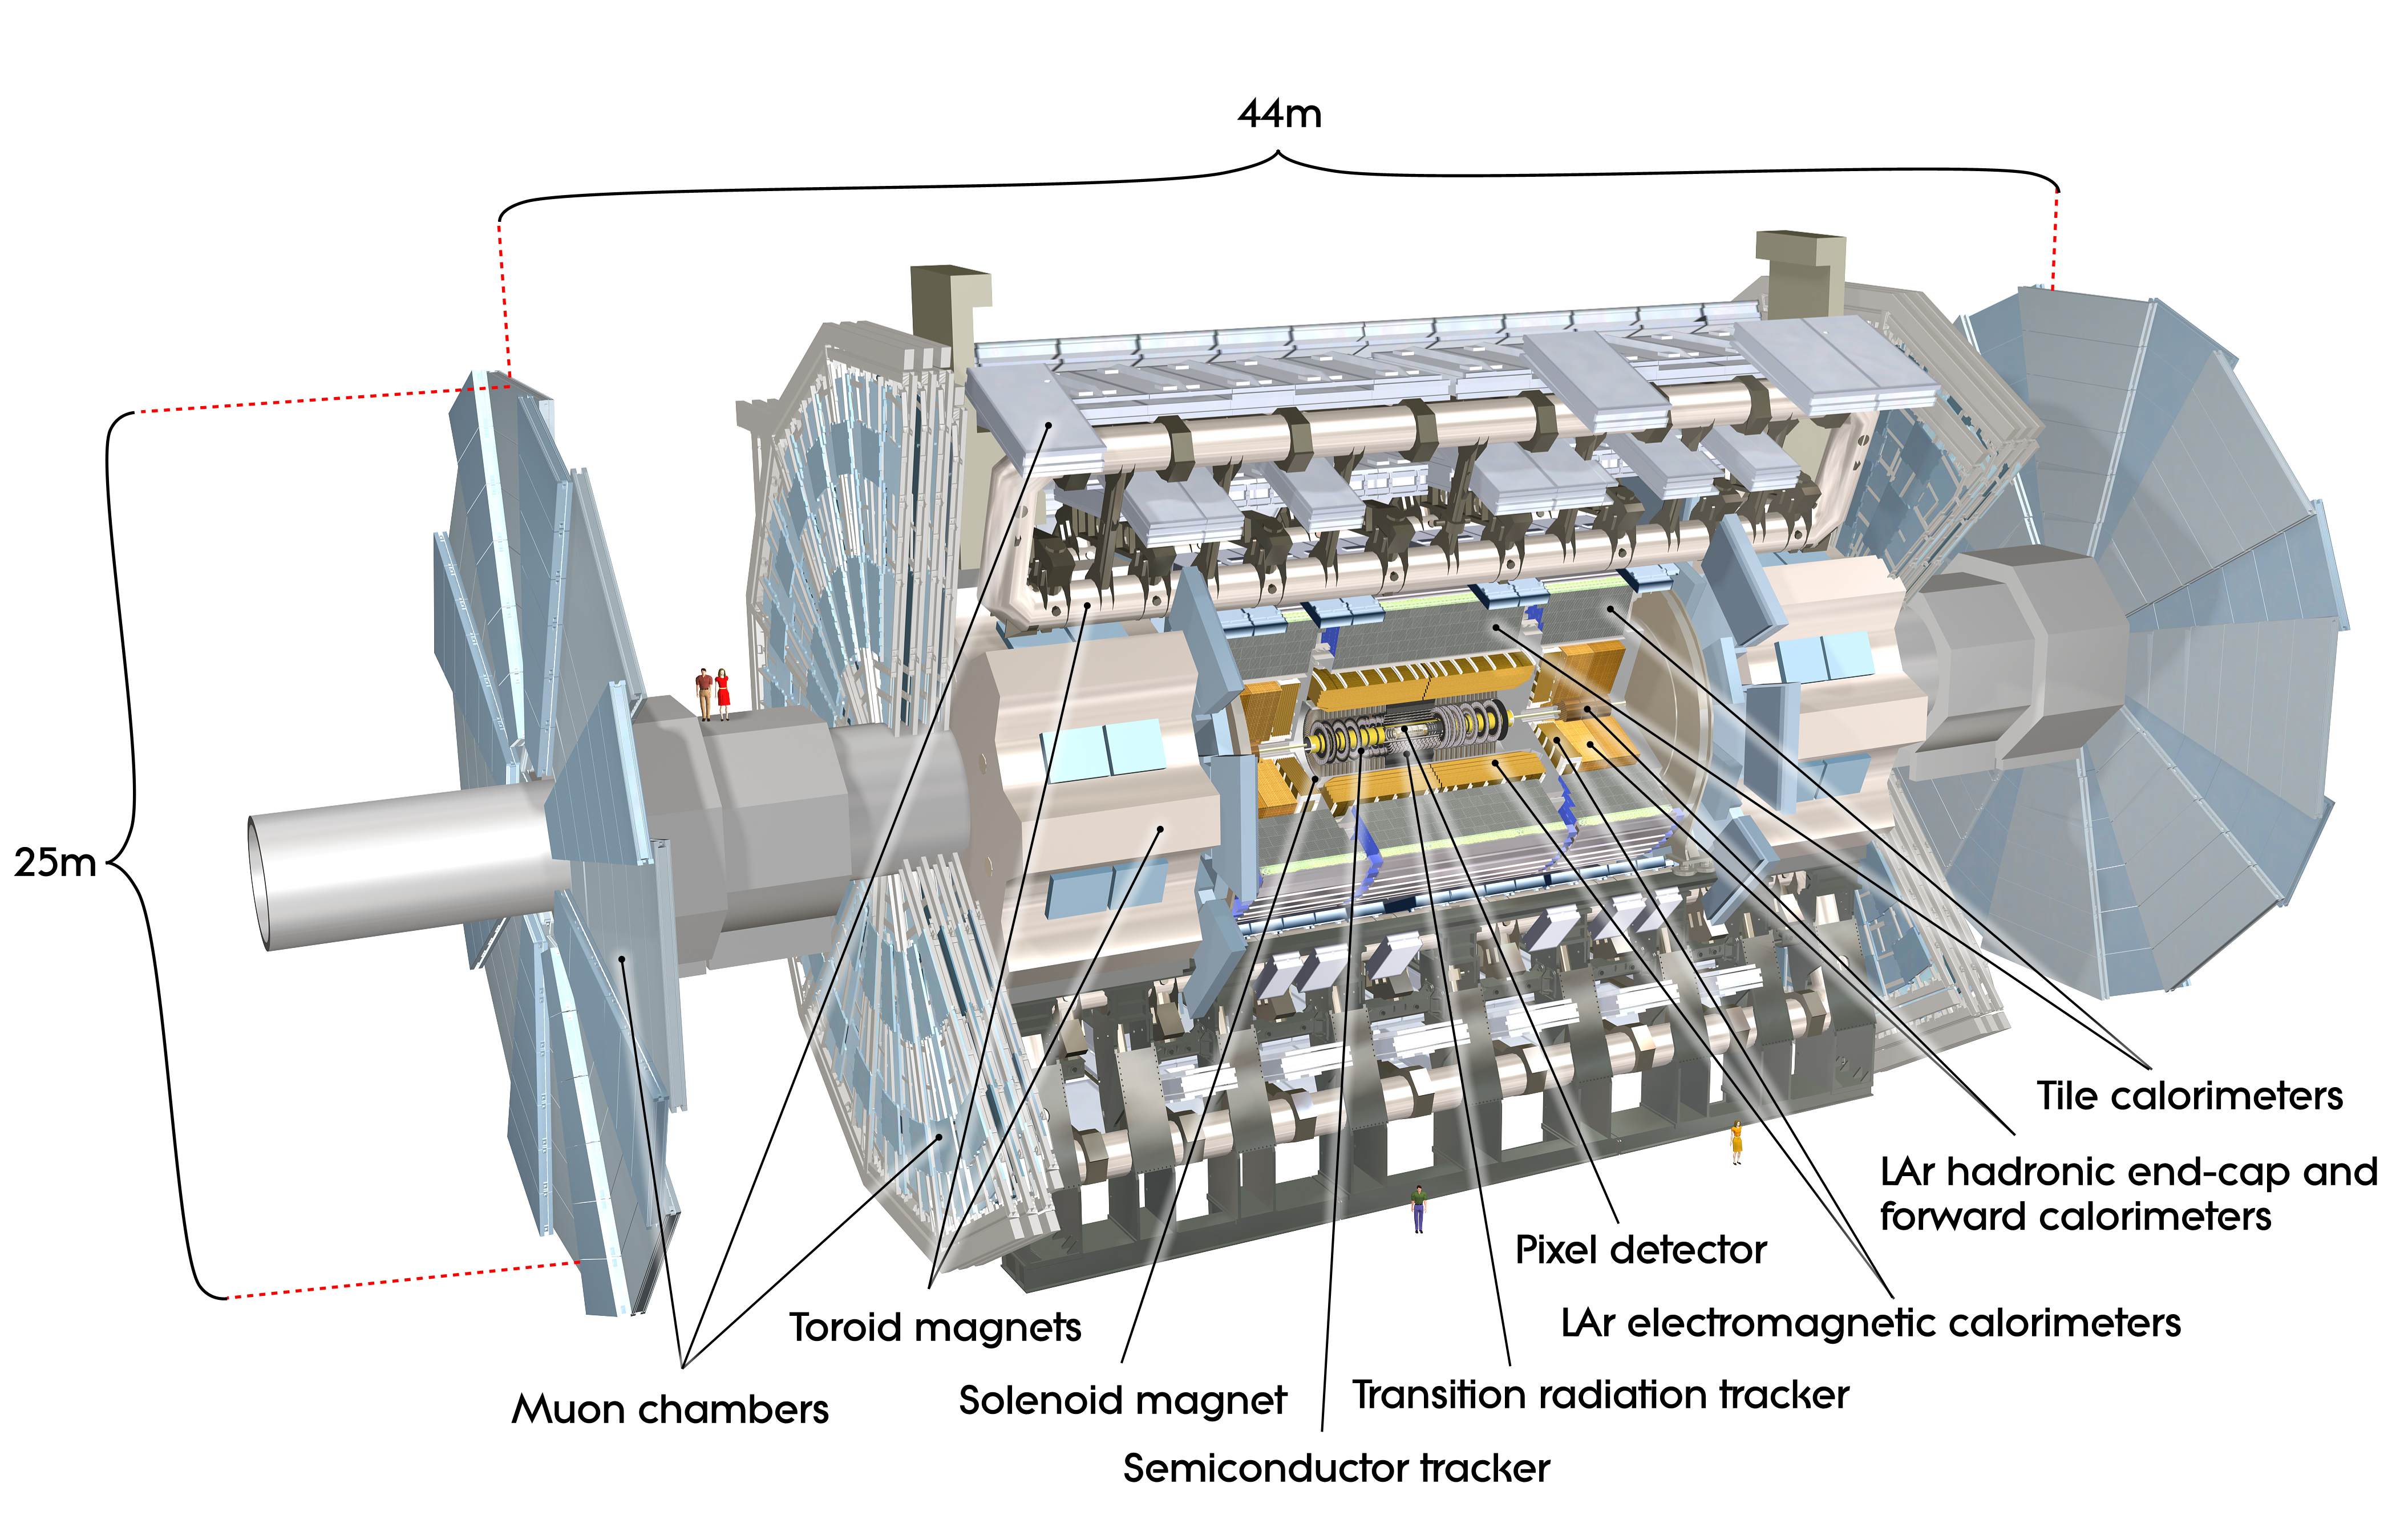
\includegraphics[width=\textwidth]{images/ATLAS.png};
    \caption[Schamatic of the ATLAS detector]{Schamatic of the ATLAS detector highlighting major 
            components within it.
            From \cite{ATLASImage} with added labels [\textbf{CITE ADAM}].}
    \label{fig:method:ATLAS}
\end{figure}

\subsubsection{ATLAS coordinate system and kinematic quantities}

ATLAS uses a right-handed coordinate system with it's origin in the center of the detector at the 
interaction point. The x-axis is aligned such that it points towards the center of the LHC ring, the positive y-axis points upwards and the z-axis is defined going along the beam-pipe. An angular system is used where \emph{r} is the radial distance from the beam line, \emph{$\phi$} is the azimuthal angle in the \emph{x-y transverse plane} and the polar angle \emph{$\theta$}. \emph{Pseudo-rapidity}, $\eta = -\log\tan\frac{\theta}{2}$ used as a dimensionless measure of \emph{$\theta$} as \emph{$\eta$} differences are invariant under Lorentz boosts to the z-axis for massless particles. The direction of reconstructed objects are defined by a measurement of $(\eta,\phi)$ and parameterisation of the distance in pseudo-rapidity angle space defined as $\eta = \sqrt{(\Delta\eta)^{2} + {\Delta\phi}^{2}}$.

The energy \emph{E} and momenta \emph{\vec{p}} of a particle can be desribed by the four-vector $P^{\mu} = (E,\vec{p})$. Whose square, $P^{\mu}P_{\mu} = E^{2} - \abs{\vec{p}^{2}}$. A Lorentz invariant mass term can be defined such that $M_{inv} = E^{2} - \abs{\vec{p}^{2}}$. Another Lorentz invariant quantity, transverse momentum \emph{$p_{T}$} is given by
\begin{equation}
    P_{T} = \sqrt{ P_{x}^{2} + p_{y}^{2}}.
\end{equation}

\subsection{Inner Detector}\label{sec:method:ID}

The Inner Detector (ID)~\cite{ATLAS:ID-TDR} embedded in a \SI{2}{\tesla} solenoid magnetic field, allows for the tracking of charged particles near to the interaction point. It is designed to achieve high precision measurements of momentum and measurements of primary and secondary vertices of collisions in the range $\abs{\eta} \leq 2.5$. It consists of in increasing distance from the beam pipe three independent detector technologies: the \emph{pixel detector}, \emph{semi-conductor tracker (SCT)} and the \emph{transition radiation tracker (TRT)}, as shown in figure \cref{fig:method:ATLAS:ID}. 

\begin{figure}
    \centering
    \begin{tikzpicture}
        \node [anchor=south west,inner sep=0] (image) at (0,0) {\includegraphics[width=\largefigwidth]{images/inner_detector}};
        \node [anchor=west] (endcap_sct) at (10,3.5) {\small End-cap SCT};
        \draw (endcap_sct) to (10.1,5.9);
        \node [anchor=west] (barrel_sct) at (8.5,2.9) {\small Barrel SCT};
        \draw (barrel_sct) to (8,4.5);
        \node [anchor=west] (pixel) at (7,2.2) {\small Pixel detector};
        \draw (pixel) to (7,4.9);
        \node [anchor=west] (barrel_trt) at (5.5,1.5) {\small Barrel TRT};
        \draw (barrel_trt) to (6.5,3);
        \node [anchor=west] (endcap_trt) at (3.5,0.8) {\small End-cap TRT};
        \draw (endcap_trt) to (4.6,2.2);
    \end{tikzpicture}
    \caption[Illustration of the ATLAS inner detector]{Illustration of the ATLAS inner detector, containing the pixel detector, semiconductor tracker (SCT), and transition radiation tracker (TRT). The \emph{insertable B-layer}, installed in 2014, is not shown. From \cite{ATLASIDImage} with added labels [REF ADAM].}
    \label{fig:method:ATLAS:ID}
\end{figure}

\subsubsection{Pixel detector}

The innermost part of the ID closest to the interaction point is the pixel detector. It provides high resolution information on the location of charged particles. Formed of four concentric cylindrical layers, the \emph{Insertable B-Layer (IBL)}~\cite{ATLAS:IBL-TDR}, added in 2014, and three additional layers in the barrel region. The layers based of silicon semiconductor technologies, detects charged particles when traversing through the doped silicon forming a electron-hole pairs resulting in a current to flow. Arranged in a grid the semiconductor sensors provide very fine granularity position information. The IBL pixels are situated at a distance of $R = \SI{33.25}{\milli\meter}$ from the centre of the beam pipe and have a size of $\SI{50}{\micro\meter} \times \SI{250}{\nano\meter}$ with an intrinsic resolution of $\SI{8}{\micro\meter} \times \SI{40}{\micro\meter}$. Whilst the outer layer pixels measure $\SI{50}{\micro\meter} \times \SI{400}{\nano\meter}$ with an intrinsic resolution of $\SI{10}{\micro\meter} \times \SI{115}{\micro\meter}$. With the addition of the IBL the resolution of primary and secondary vertices was improved to \SI{10}{\nano\meter} in R$\phi$ and \SI{115}{\micro\meter} in z~\cite{Rosa}. 

\subsubsection{Semiconductor tracker}
Based on silicon sensors the SCT is located \SI{299}{\nano\meter} from the interaction point. However, it uses \SI{128}{\milli\meter} long strips of sensors with relatively large extend in z. It detects charged particles through the same mechanism as the pixel detector, however, with a lower granularity. The SCT strip modules are arranged in pairs with a \SI{40}{\milli\radian} relative angle, where each modules consists of a number of SCT strips. Therefore providing two independent hits allowing for the measurement of $(r,\phi)$ without requiring individual pixel hits. Four cylindrical layers surround the pixel detector in the barrel region and nine disks in the end-caps. Therefore, in the barrel region for each track, four space points with an intrinsic resolution of \SI{17}{\micro\meter} in R$\phi$ and \SI{580}{\micro\meter} in z can be obtained.

\subsubsection{Transition radiation tracker}
Located \SI{563}{\milli\meter} from the interaction point the TRT is the outermost component of the ID. The TRT is formed of approximately 370000 gas filled straw tube detectors. Each straw tube is a hollow cylinder with a diameter of \SI{4}{\milli\meter} containing a central tungsten wire filled with a gas mixture of 70\% Xe, 27\% CO$_{2}$ and 3\% O$_{2}$. The tungsten wire along with the tube forms a capacitor, where the wire is the anode and the surrounding tube acts as the cathode. When charged particles pass through the tube, the gas is ionised producing a cascade of electrons. These electrons are attracted to the anode creating a current in the wire. The TRT has 73 straw planes in the barrel region, spaced horizontally at a distance $\SI{563}{\milli\meter} < R < \SI{1066}{\milli\meter}$ and $\abs{z} < \SI{712}{\milli\meter}$ from the interaction point, and 160 straw planed in the end-caps orientated in the radial direction. This results in on average 30 to 40 hits detected per particle by the TRT. The TRT straws have an intrinsic resolution of \SI{130}{\micro\meter} in the $R\phi$ plane. 

The TRT additionally consists of polypropylene fibres and polypropylene foils interleaved between the straw tubes in the barrel and endcap modules respectively. Charged particles passing through the polypropylene undergo transition ration. Transition radiation is produced when particles travel between materiels with different dielectric constants. The radiation results in additional ionisation of the gas in the straw tubes. The energy of the transition radiation is dependant upon mass of the charged particles, which allows for a separation of from electrons and from other charged particles.  

\subsubsection{Performance}

Precise tracking information is needed to measure the properties of particles expected in final states of analyses. Using the information from the ID with the exclusion of the IBL, the expected resolution is given by [REF]
\begin{equation}
   \sigma(\frac{1}{p_{T}}) \cdot p_{T} = 0.036 \% \cdot p_{T}[GeV] \oplus 1.3 \%
\end{equation}

\subsection{Calorimeters}\label{sec:method:Cals}
The ATLAS calorimetry system consists of the electromagnetic and the hadronic calorimeters, located closest to the beam pipe after the ID outside of the solenoid magnet. Designed to measure the position and energy of particles emerging from the interaction point. Using materials which have a high probability of particles interaction with them, the electromagnetic and hadronic calorimeters are specialised in measuring the energies of $\gamma$ and $e$, and hadrons, respectively. Neutral particles like $\gamma$ and neutral hadrons which do not induce a signal in the ID can be identified in the calorimeters. This allows for nearly all Standard Model particles to be identified with the exception of weakly interaction neutrinos and $\mu$ which has minimal ionization within the distance of the calorimeters and the interaction point. 

High energy particles undergo multiple scattering producing a \emph{shower} of lower energy particles that travel through the calorimeter material. Therefore, it is important to ensure that  \emph{particle showers} are contained within the calorimeters when designing them. The depth of a calorimeter material can be characterised by a particles radiation lengths ($\chi_{0}$) and it's nuclear interaction lengths ($\lambda$). Nuclear interaction length is be defined as the mean distance a particle travels in a medium before undergoing inelastic scattering. Due to electromagnetic interactions with the surrounding material, over one radiation length a particle loses on average $e^{-1}$ it's original energy. 

ATLAS using sampling calorimeters for both the electromagnetic and hadronic calorimeters. The Calorimeter materials have been selected to either be ionised or scintillate when particle a particle shower enters which results in a measurable electrical signals. A particles energy can be calculated by summing the total radiation produced by a shower in the active layers. 

\subsubsection{Electromagnetic calorimeter}
The electromagnetic calorimeter is designed to fully measure the energies of electrons (and positrons), and photons. Measurements of the particles energies are made by inducing electromagnetic showers when the particle interacts with a dense material. For electrons the shower is primarily initiated by bremsstrahlung, whilst for photons it is initiated by pair production. Shower particles are then be detected by the detecting layers of the calorimeter interleaved with layers of dense material.

\begin{figure}
    \centering
    \begin{tikzpicture}
        \node[anchor=south west,inner sep=0] (image) at (0,0) {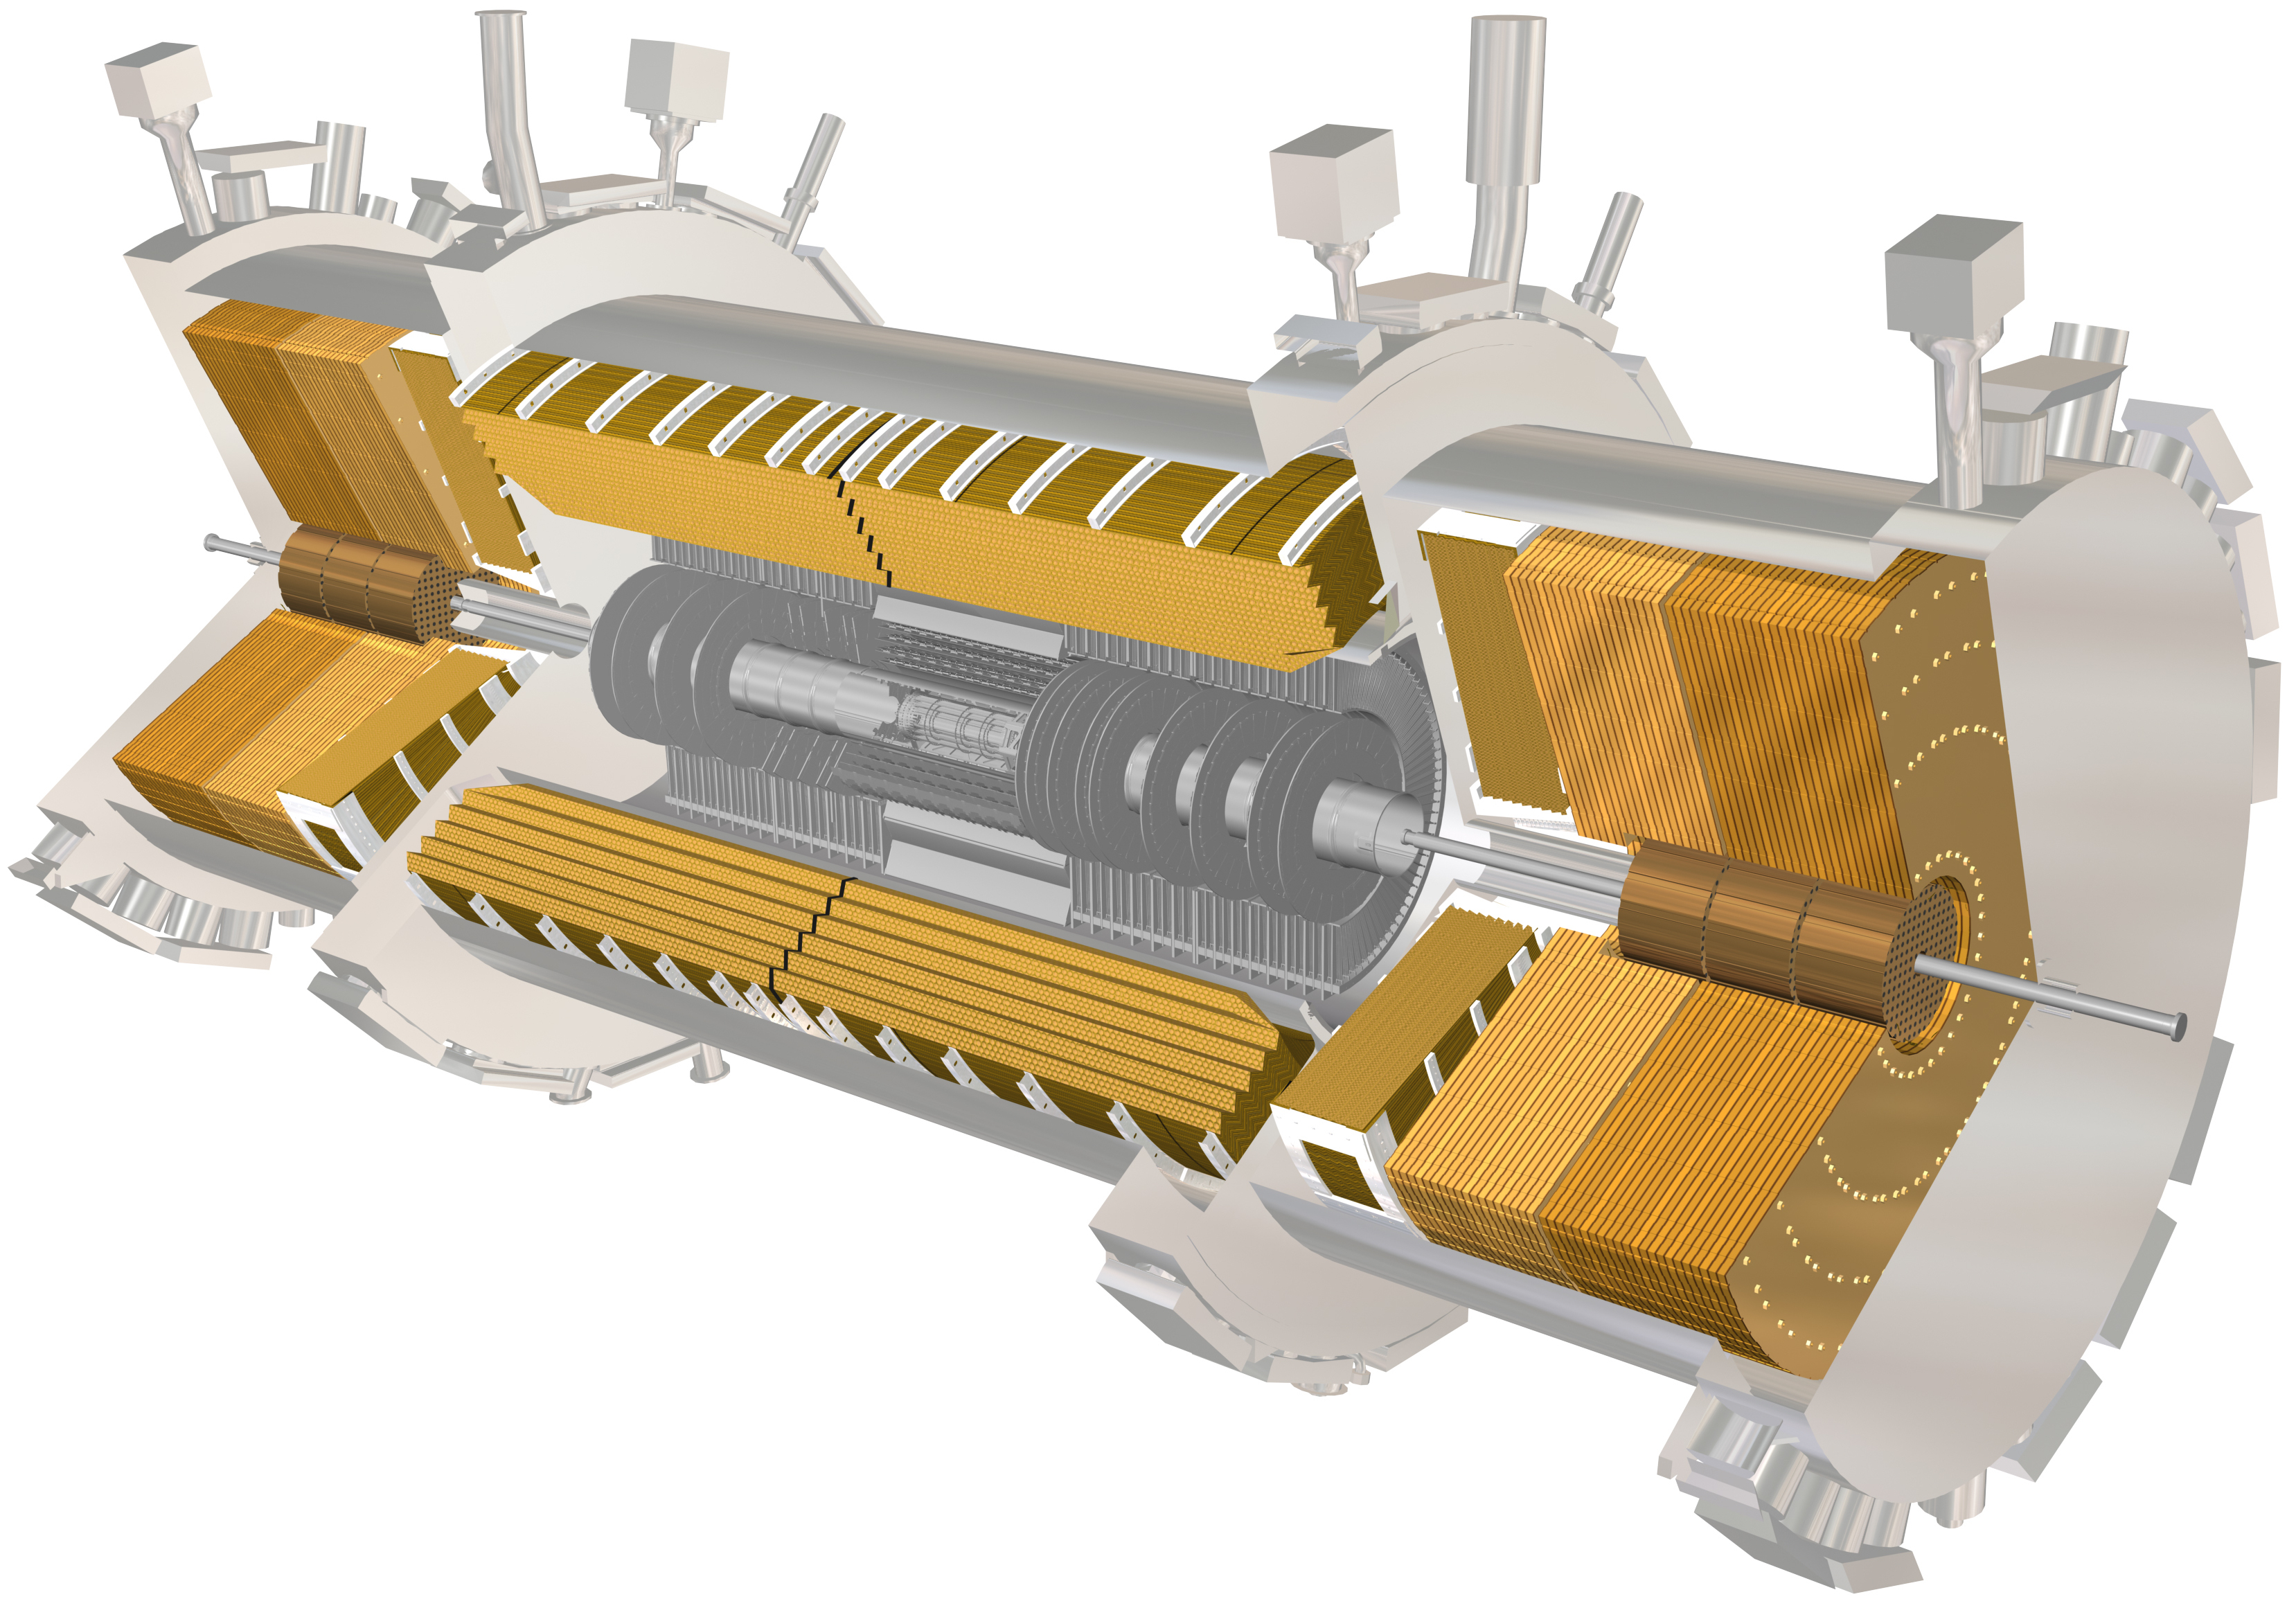
\includegraphics[width=\largefigwidth]{images/lar}};
        \node[anchor=west,align=center] (hec) at (-2.0,2.3) {\small Hadronic end-cap\\ calorimeter};
        \draw (hec) to ++(2,2.5);
        \node[anchor=west,align=center] (fcal) at (8.5,-0.8) {\small Forward calorimeter};
        \draw (fcal) to ++(-1.4,4.4);
        \node[anchor=west,align=center] (ecal) at (0,1) {\small Barrel electromagnetic\\ calorimeter};
        \draw (ecal) to ++(1.3,2.6);
        \node[anchor=west,align=center] (emec) at (4,0) {\small Electromagnetic end-cap\\ calorimeter};
        \draw (emec) to ++(1.1,3);
        \clip (current bounding box.south west) rectangle ($(current bounding box.north east)+(1.5,0)$);
    \end{tikzpicture}
    \caption[Illustration highlighting the liquid argon components of the ATLAS calorimeters]{Illustration highlighting the liquid argon components of the ATLAS calorimeters.
        From \cite{ATLASLarImage} with added labels.}
    \label{fig:method:ATLAS:LAr}
\end{figure}

The electromagnetic calorimeter uses liquid argon (LAr) as it's scintillator material and lead plates as it's shower inducing material. Liquid argon component of the colorimeter were chosen due to it's stability of response over a long period of time whilst being exposed to radiation~\cite{ATLAS:LAr-TDR}. It's divided into barrel and end-cap regions highlighted in \cref{fig:method:ATLAS:LAr}. 

In the barrel region the electromagnetic calorimeter is split into three regions of different granularity. The innermost layer of the calorimeter has a fine granularity in $\eta$. Majority of the thickness of the electromagnetic calorimeter consists of the second layer, arranged in a square grid, aids in locating the primary vertices of particles. Combining the measurements of the first two layers allows for locating the origin of neutral particles, which do not leave tracks in the ID. The final layer, with the largest granularity, is used to estimate the energy lost beyond the electromagnetic calorimeter and to distinguish between electromagnetic and hadronic showers. A sketch of the barrel module can be seen in \cref{fig:method:ATLAS:ECal}, where the cell granularity of each section is clearly visible.
\begin{figure}
    \centering
    \begin{tikzpicture}
        \node[anchor=south west,inner sep=0] (image) at (0,0) {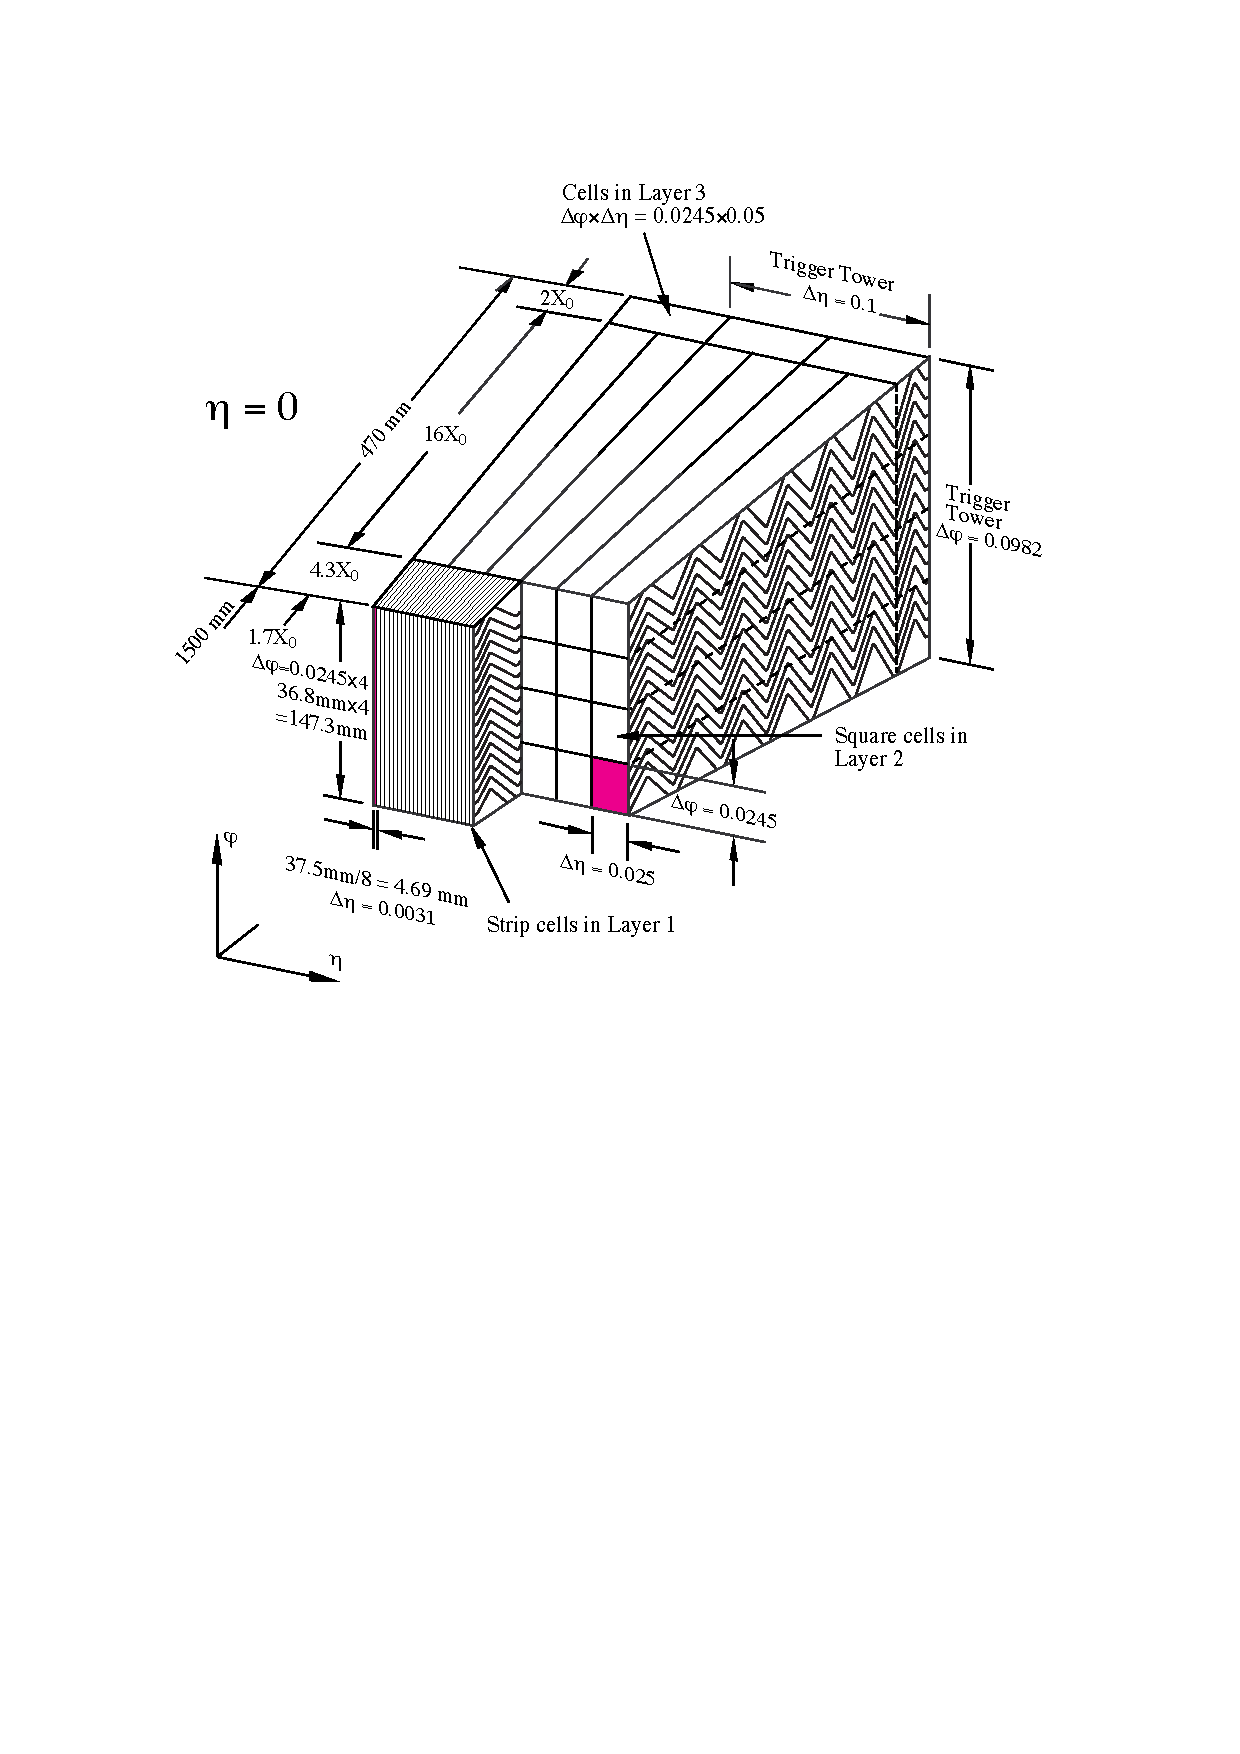
\includegraphics[scale=0.9]{images/calo.pdf}};
    \end{tikzpicture}
    \caption[Drawing showing a section of the barrel electromagnetic calorimeter]{Drawing showing a section of the barrel electromagnetic calorimeter.
    The liquid argon cells are arranged into three distinct layers, with granularity decreasing for larger radius.
    From \cite{ATLAS}.}
    \label{fig:method:ATLAS:ECal}
\end{figure}

In the forward region, each end-cap electromagnetic calorimeter consists of two coaxial wheels separated by \SI{3}{mm}. The inner wheels are constructed similarly to the barrel calorimeters shown in \cref{fig:method:ATLAS:ECal}. The other wheels do not have a third layer and majority of the thickness is composed of the first two layers. 

\subsubsection{Hadronic calorimeter}
The hadronic calorimeter, like the electromagnetic one, is a sampling calorimeter. Unlike the electromagnetic calorimeter it uses steel as the shower-inducing material and plastic scintillating tiles~\cite{ATLAS:tile-TDR}. The tile calorimeter sits in the barrel region at $\abs{\eta} < 1.7$ where it divided into, the tile barrel $\abs{\eta} < 1.0$ followed by the extended barrels covering $ 0.8 < \abs{\eta} < 1.7 $. The barrel and extended barrels are divided azimuthally into 64 modules. On the edges of the tiles wavelength shifting fibers are extract signals by guiding them into photomultiplier tubes. 

The hadronic end-cap calorimeter covers  $1.5 < \abs{\eta} < 3.2$ using LAr technology. It consists of two wheels per end-cap, and uses copper as the shower inducing material. In each end-cap it two independent wheels are placed with \SI{50}{\milli\meter} copper plates. A greater containment is achieved compared to the tile calorimeter by placing 12 nuclear interaction lengths of material before the muon spectrometers. 

\subsubsection{Forward calorimeters}
The forward calorimeter provides additional coverage in the range $3.1 < \abs{\eta} < 4.9$ and is designed to measure the energies of both electromagnetic and hadronic showers~\cite{ATLAS:LAr-TDR}. It consists of three modules, each using LAr as the detecting material. Copper rods are placed parallel to the beam axis in the innermost layer, is optimised for electromagnetic showers. Tungsten rods are used for the second and third layers as the shower inducing material to measure the energy of hadronic particles. 

\subsubsection{Performace}

Many analysis in ATLAS require an excellent energy resolution. Based on test beam data, the calorimeter the calorimeter energy resolution is summarized in Table ~\cite{ATLAS:testbeam-calo}~\cite{ATLAS:testbeam-hcal}.

\begin{table}
    \begin{tabular}{ccc}
         & jet \pT [\si{\giga\eV}] & Resolution \\
        \midrule
        $\geq 6$ & $\frac{\sigmaE}{E} =$ \\
        $\geq 5$ & $>65$ & $\geq 0$ & $240\,166 \pm 412$ \\
        $\geq 2$ & $>75$ & $\geq 2$ & $303\,399 \pm 464$ \\
    \end{tabular}
    \caption[Comparison of trigger strategies]{Comparison of trigger strategies.
        The minimum number of jets, \pT for those jets, and number of \Pbottom-tagged jets are shown with the associated yields after applying to Monte Carlo simulation.
        The top row corresponds to the strategy used for the analysis in this chapter.}
    \label{tab:analysis:trigger-yields}
\end{table}

\subsection{Muon spectrometer}\label{sec:method:MS}

\subsection{Trigger and Data Acquisition System}